\FloatBarrier
\section{The Block Power Method}
\label{sec:numerics}
\label{sec:nonhermitian}

Section~\ref{sec:transverse} reduced the dynamics to the leading eigenpairs of the transfer matrix $\mathcal{E}$. This section presents the algorithm we use to obtain them: a block power method that iterates several temporal states at once and returns the dominant eigenvalues together with their left and right eigenvectors, identified and ordered for the comparison with the \ac{CFT} predictions. The implementation details are collected in Appendix~\ref{app:blockpm}.

The right and left eigenvectors of $\mathcal{E}$ satisfy
\begin{equation}
  \mathcal{E}\ket{R_i}=\mu_i\ket{R_i},
  \qquad
  \bra{L_i}\mathcal{E}=\mu_i\bra{L_i}.
  \label{eq:nonhermitian_eigenproblem}
\end{equation}
Because $\mathcal{E}$ is non-normal (Section~\ref{sec:mporep:fsm}), the left and right eigenvectors are different objects, and neither set is orthogonal on its own; instead, the two sets are biorthogonal, $\braket{L_i}{R_j}\propto\delta_{ij}$. The bra notation involves no conjugation: $\bra{L_i}$ is a row vector, and $\braket{L_i}{R_j}$ is the direct contraction of the two temporal networks. Numerically, the left states are propagated with the transpose $\mathcal{E}^{\mathsf T}$, which is the matrix form of the left equation above.

The dominant eigenvalue $\mu_0$ carries the Loschmidt rate in its modulus and the central charge in its phase, the gaps to the subleading eigenvalues carry the boundary operator content, and the generalized temporal entropies are built from the dominant pair $(\bra{L_0},\ket{R_0})$. The calculation must therefore resolve the leading eigenvalues individually, identify $\mu_0$ among them, and order the rest so that they can be matched to the conformal tower; how this is done is described in Section~\ref{sec:reach}.

\subsection{The block power method}
\label{sec:blockpm}

A single-vector power method converges at a rate set by $|\mu_1/\mu_0|$, and stalls once that ratio approaches one. This is the regime the conformal predictions apply in, since the leading eigenvalues approach a common modulus as $T$ grows. Iterating a block of $k$ states avoids the difficulty. The block converges to the leading $k$-dimensional invariant subspace at a rate set by $|\mu_{k+1}/\mu_k|$, so near-degenerate eigenvalues inside the block no longer limit it. They are separated afterwards by the projected eigenproblem below.

The block method evolves $k$ right \acp{tMPS}, $\{\ket{R_1},\dots,\ket{R_k}\}$, together with $k$ left \acp{tMPS}, $\{\bra{L_1},\dots,\bra{L_k}\}$. The two blocks are initialized independently with random complex tensors. Algorithm~\ref{alg:blockpm} summarises one iteration, while Figure~\ref{fig:blockpm} shows the tensor-network operations involved in applying and projecting the transfer matrix.

\begin{figure}[htbp]
  \centering
  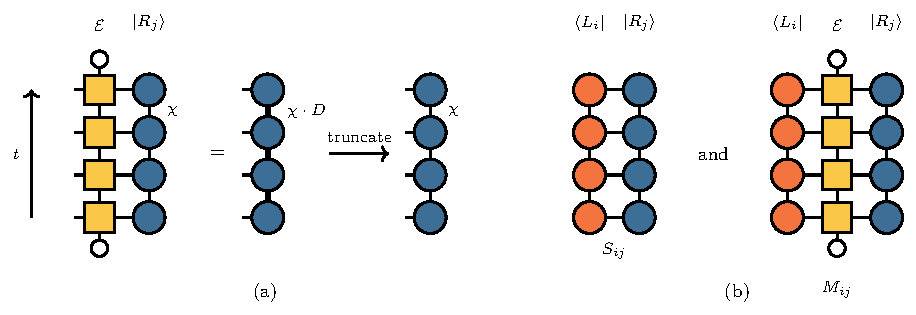
\includegraphics[width=0.8\textwidth]{imgs/blockpm.pdf}
  \caption{\textbf{One iteration of the block power method.} Each \ac{tMPS} is a column, and $\mathcal{E}$ is the corresponding column of the space--time network, closed at both ends by the product state (small open circles). (a) Application of $\mathcal{E}$ to one member of the right block, Eq.~\eqref{eq:blockpm_apply}: the temporal bond dimension grows from $\chi$ to $\chi \cdot D$, with $D$ the \ac{tMPO} bond dimension, and is truncated back to $\chi$. The left block is treated analogously with the transpose. (b) The contractions defining the two $k\times k$ matrices of Eq.~\eqref{eq:blockpm_pencil}; the left chain enters directly as a bra, without conjugation.}
  \label{fig:blockpm}
\end{figure}

\begin{algorithm}[H]
\caption{\textbf{Block power method} for the $k$ dominant eigenpairs of $\mathcal{E}$.}
\label{alg:blockpm}
\begin{algorithmic}[1]
\State $\ket{R_j},\ \bra{L_j} \gets$ random complex \acp{tMPS}, \quad $j=1,\dots,k$
\Repeat
  \State $\ket{\tilde R_j} \gets \operatorname{truncate}_\chi\big(\mathcal{E}\ket{R_j}\big)$, \qquad $\bra{\tilde L_j} \gets \operatorname{truncate}_\chi\big(\bra{L_j}\,\mathcal{E}\big)$ \Comment{apply}
  \State $S_{ij} \gets \braket{L_i}{R_j}$, \qquad $M_{ij} \gets \braket{L_i}{\tilde R_j}=\bra{L_i}\mathcal{E}\ket{R_j}$ \Comment{project}
  \State solve $M v=\theta\,S v$ for Ritz values $\theta_1,\dots,\theta_k$ and coefficients $V$, $U$
  \State $\ket{R_j} \gets \operatorname{truncate}_\chi\big(\textstyle\sum_i V_{ij}\ket{\tilde R_i}\big)$, \qquad $\bra{L_j} \gets \operatorname{truncate}_\chi\big(\textstyle\sum_i U_{ij}\bra{\tilde L_i}\big)$ \Comment{de-mix}
  \State normalize every block member
\Until{the leading Ritz values stop changing within tolerance}
\end{algorithmic}
\end{algorithm}

The first step applies the transfer matrix to each member of the right block and its transpose to each member of the left block,
\begin{equation}
  \ket{\tilde R_j} = \mathcal{E}\ket{R_j},
  \qquad
  \bra{\tilde L_j} = \bra{L_j}\,\mathcal{E}
  \;\;\Longleftrightarrow\;\;
  \ket{\tilde L_j} = \mathcal{E}^{\mathsf T}\ket{L_j}.
  \label{eq:blockpm_apply}
\end{equation}
Applying the \ac{tMPO} multiplies the bond dimension of each state by the \ac{tMPO} bond dimension $D$, as shown in Figure~\ref{fig:blockpm}a. We therefore truncate each propagated state back to the maximum bond dimension $\chi$ using either scheme of Section~\ref{sec:transverse:truncation}, and then normalize it. The truncation cannot be deferred to the end of the sweep: without it the bond dimension is multiplied by $D$ at every iteration, so the cost of the next application would grow geometrically. Truncating after the de-mixing step instead of before it would be equivalent, but it would require holding $k$ states of dimension $\chi D$ simultaneously.

The next step projects the eigenproblem onto the current block subspaces. We approximate a right eigenvector by
\begin{equation}
  \ket{\psi} = \sum_{j=1}^{k} v_j \ket{R_j}.
  \label{eq:blockpm_ansatz}
\end{equation}
This approximation leaves a residual when inserted into $\mathcal{E}\ket{\psi}=\theta\ket{\psi}$. Requiring the residual to vanish against every member of the left block gives $\bra{L_i}(\mathcal{E}-\theta)\ket{\psi}=0$. The full eigenproblem is thereby reduced to the two $k\times k$ matrices shown in Figure~\ref{fig:blockpm}b,
\begin{equation}
  S_{ij}=\braket{L_i}{R_j},
  \qquad
  M_{ij}=\bra{L_i}\mathcal{E}\ket{R_j},
  \label{eq:blockpm_pencil}
\end{equation}
and the generalized eigenvalue problem
\begin{equation}
  \sum_{j} M_{ij}\,v_j = \theta \sum_{j} S_{ij}\,v_j .
  \label{eq:blockpm_smallproblem}
\end{equation}
The overlap matrix $S$ measures the relative orientation of the left and right subspaces, while $M$ is the transfer matrix projected between them. Solving Eq.~\eqref{eq:blockpm_smallproblem} returns the Ritz values $\theta_j$ together with two sets of coefficients. The right eigenvectors $V$ of the $k\times k$ pencil say how to combine the propagated right states into one approximate eigenvector each, and the left eigenvectors $U$ do the same for the left block. These are the $V$ and $U$ of Algorithm~\ref{alg:blockpm}. The resulting Ritz values approximate $\mu_0,\dots,\mu_{k-1}$, and the coefficient matrices identify the corresponding combinations within each block. If $S$ becomes ill-conditioned, the oblique projection amplifies numerical errors, so we solve Eq.~\eqref{eq:blockpm_smallproblem} with the pseudoinverse regularization described in Appendix~\ref{app:blockpm}.

The Ritz coefficient matrices are then used to de-mix the propagated blocks, assigning each member to one approximate eigenpair. The resulting states are truncated back to $\chi$ and normalized before the next iteration. We stop when the leading Ritz values remain stable within the prescribed tolerance.

The computational cost is dominated by the tensor-network operations rather than the $k\times k$ eigenproblem. Each iteration requires $2k$ applications of the \ac{tMPO}. De-mixing is usually more expensive still, because it first combines $k$ \acp{tMPS}, which multiplies the bond dimension by $k$, and only then compresses the result. Appendix~\ref{app:blockpm:cost} quantifies this breakdown and the measures that reduce it.

When only the eigenvalues are needed, we do not assign individual block members to separate eigenvectors at all. The blocks are kept in an orthonormal Schur basis of the leading invariant subspace, updated by a QR decomposition of the coefficient matrices (Appendix~\ref{app:blockpm:schur}). No accuracy is lost, because the Ritz values do not depend on the basis chosen inside the blocks. Recombining the blocks by any invertible $B$ and $C$ sends $S\to B^{\mathsf T}SC$ and $M\to B^{\mathsf T}MC$, which leaves the solutions of Eq.~\eqref{eq:blockpm_smallproblem} unchanged. The two modes read the same spectrum from the same pair of subspaces, and differ only in how well conditioned the basis is when it is truncated. That favours the orthonormal one, since the eigenvector coefficients become ill-conditioned where the block is near-degenerate. We use this mode for the late-time spectral measurements in Section~\ref{sec:results}.

It is worth mentioning that the truncation at each iteration uses only the current states, not the columns of the network still to be absorbed, so a component discarded now could in principle matter later. Translation invariance keeps this harmless: every subsequent column applies the same operator $\mathcal{E}$, which regenerates any part of the leading invariant subspace that has been trimmed away.

Finally, we validate the implementation at bond dimensions for which $\mathcal{E}$ can be constructed explicitly and diagonalized exactly. Across the models tested, the block method reproduces the leading dense spectrum with errors between $10^{-8}$ and $10^{-13}$. The corresponding tests are reported in Appendix~\ref{app:blockpm:validation}.

\subsection{Selecting the physical branch and testing convergence}
\label{sec:reach}

The block returns $k$ Ritz values at each evolution time, and the physical $\mu_0$ has to be identified among them. We take the eigenvalue of largest modulus, and use continuity with the preceding rung to break the tie when two moduli agree to within one per cent. Such ties are produced by the conformal spectrum itself: as $T$ grows the moduli of the tower states approach a common value, which is the emergent dual unitarity of Section~\ref{sec:cft:temporal}. The subleading eigenvalues are then ordered by their phase distance from $\mu_0$, the order in which the conformal tower arranges them. Appendix~\ref{app:selector} records the full procedure and its safeguards.

Eigenvalues and eigenvectors then lose accuracy at different points, which determines how far each measurement can be trusted. First-order perturbation theory for a non-Hermitian matrix~\cite{wilkinson1965} gives the two sensitivities, and they differ (Appendix~\ref{app:conditioning}). The shift of an eigenvalue is controlled by its own biorthogonal overlap $\braket{L_j}{R_j}$ and involves no eigenvalue difference. The mixing of an eigenvector with its neighbours is divided by $\mu_i-\mu_j$, so it grows as soon as two eigenvalues approach. Eigenvalues therefore survive past the point where the eigenvectors, and any quantity built from them, have stopped being meaningful. The remaining protection is measured by the phase rigidity of a biorthogonal pair,
\begin{equation}
    r_j = \frac{|\braket{L_j}{R_j}|}{\lVert L_j\rVert\,\lVert R_j\rVert},
    \label{eq:rigidity}
\end{equation}
the normalized overlap between the left and right eigenvector of the same eigenvalue. For a Hermitian matrix the two coincide and $r_j=1$; as the left and right eigenvectors of a non-normal matrix rotate towards a common direction, $r_j$ falls towards zero. We monitor it as the conditioning diagnostic of the eigenvector route (Appendix~\ref{app:conditioning}).

Finally, we test whether an observed limitation is physical or resolution dependent by repeating representative calculations at half the bond dimension, with a tighter truncation cutoff, and with \ac{RDM} rather than \ac{RTM} truncation. We attribute a feature to the transfer matrix only if it persists under all three changes.

\subsection{Universal versus non-universal constants}
\label{sec:numerics:universal}

The predictions of Section~\ref{sec:cft} are exact only in the continuum limit. A simulation instead runs on a microscopic lattice, at finite evolution time $T$, bond dimension $\chi$ and Trotter step $\delta t$, and with a nonzero regulator $\beta_0$. Its measurements therefore mix two kinds of contributions. The universal ones are fixed by the universality class: the central charge $c$ and the scaling dimensions $x_i$, which set every coefficient in Eqs.~\eqref{eq:cft:chord}--\eqref{eq:gapclose}. The non-universal ones are introduced by the lattice and the algorithm: the regulator $\beta_0$ and the entropy offset $s_0$ it feeds, the Trotter step $\delta t$, the sound velocity $v$, and the overall normalization of the transfer matrix, which is model dependent and makes the modulus of the dominant eigenvalue differ from one. How well these contributions can be separated determines which predictions can be compared with a simulation and how that comparison should be made.

The sound velocity is non-universal, but it can be measured independently from the equilibrium dispersion of the same model (Section~\ref{sec:annni:velocity}). Since the eigenvalue phases depend on the combination $\pi x/(vT)$, the velocity is needed to convert a measured phase gap into the corresponding universal scaling dimension $x_i$.

This separation is possible because the universal and non-universal contributions affect the spectrum differently. The transfer matrix carries an overall normalization that the lattice construction fixes and the continuum theory does not. Each column of the network is one Trotter layer together with the cooling rows, so its scale depends on $\delta t$, on $\beta_0$, and on the normalization convention chosen for the local \ac{MPO} tensor. Its closed form is not needed: the constant multiplies every eigenvalue alike, so it rescales all the moduli $|\mu_i|$ and leaves the phases untouched. The universal level structure therefore appears in the phases, and we read scaling dimensions from phase differences, using the moduli only through ratios or their limiting behaviour.

Ratios remove more than the normalization. A single phase gap contains a universal dimension, but also depends on the regulator $\beta_0$ and the velocity. The ratio of two gaps,
\begin{equation}
    \frac{\mathrm{Im}(\lambda_2-\lambda_0)}{\mathrm{Im}(\lambda_1-\lambda_0)}
      = \frac{x_2-x_0}{x_1-x_0},
    \label{eq:cft:gapratio}
\end{equation}
is independent of all three at once, since $\beta_0$, the velocity and the normalization cancel between numerator and denominator. It therefore probes the operator content without any external input and provides the cleanest measurement available to us.

Not every quantity can be turned into a ratio of this kind. The entropy slope of Eq.~\eqref{eq:cft:chord} measures $c$ directly, but at finite $(T,\chi,\delta t)$ the measured slope is the continuum coefficient multiplied by a correction factor,
\begin{equation}
  \mathrm{slope}(p) = \frac{c(p)}{8}\,K(T,\chi,\delta t,\beta_0),
  \label{eq:cft:calib}
\end{equation}
where $K$ collects the finite-time, truncation and Trotter corrections, which two models in the same universality class share when run through the same pipeline at matched parameters. The integrable point of the chain makes this factor measurable: there $c=\tfrac12$ exactly, so the measured $\mathrm{slope}(0)$ determines $K$ itself. Dividing the two slopes then cancels it,
\begin{equation}
  c(p) \approx \frac{1}{2}\,\frac{\mathrm{slope}(p)}{\mathrm{slope}(0)}.
  \label{eq:cft:calibratio}
\end{equation} The cancellation is exact only for corrections common to both runs. It therefore assumes that the two models share a universality class, which is part of what the measurement is meant to establish. Coupling-dependent subleading terms do not cancel and set the residual uncertainty. The calibrated number is a consistency check rather than an independent determination. The second route uses the fact that the functional form of the corrections is itself fixed by the \ac{CFT}~\cite{boucomas2026}, so they can be included explicitly in the fit and $c$ extracted absolutely, without a reference. The costs differ: the absolute route needs a window in $T$ long enough to separate the correction from the leading term, while calibration works at shorter times but needs the reference simulation.